\documentclass[tikz,border=6pt]{standalone}

\usepackage[T1]{fontenc}
\usepackage[utf8]{inputenc}
\usepackage{helvet}
\renewcommand{\familydefault}{\sfdefault}
\usepackage{tikz}
\usetikzlibrary{arrows.meta,fit,backgrounds,calc}

\definecolor{noirbg}{HTML}{131B24}
\definecolor{noirpanel}{HTML}{1C2834}
\definecolor{noirpanelalt}{HTML}{2A3948}
\definecolor{noirline}{HTML}{556779}
\definecolor{noirtext}{HTML}{ECF1F4}
\definecolor{noirmuted}{HTML}{C4CDD5}
\definecolor{duneorange}{HTML}{F2682B}
\definecolor{noircyan}{HTML}{92DDF2}
\definecolor{noirmint}{HTML}{96D6AE}

\tikzset{
  stage/.style={
    draw=noirmuted,
    rounded corners=4pt,
    semithick,
    minimum height=1.15cm,
    align=center,
    font=\sffamily\footnotesize,
    fill=noirpanel,
    text=noirtext,
    inner sep=6pt
  },
  hot/.style={stage, draw=duneorange, very thick, fill=noirpanelalt},
  future/.style={stage, draw=noirmint, very thick, fill=noirpanelalt},
  shared/.style={stage, draw=noircyan, semithick},
  reject/.style={
    rounded corners=10pt,
    semithick,
    minimum height=0.75cm,
    align=center,
    font=\sffamily\scriptsize,
    fill=noirpanel,
    text=noirtext,
    inner sep=4pt
  },
  callout/.style={
    rounded corners=4pt,
    semithick,
    fill=noirbg,
    align=center,
    font=\sffamily\scriptsize,
    text=noirmuted,
    inner sep=4pt
  },
  flow/.style={-{Latex[length=2.4mm]}, thick, draw=noirmuted},
  accent/.style={-{Latex[length=2.2mm]}, semithick, draw=duneorange},
  subtle/.style={-{Latex[length=2.0mm]}, semithick, dashed, draw=noircyan},
  rowlabel/.style={font=\sffamily\small\bfseries, text=noirtext, fill=noirbg, inner sep=1.5pt},
  collabel/.style={font=\sffamily\scriptsize\bfseries, text=noirmuted}
}

\begin{document}
\pagecolor{noirbg}
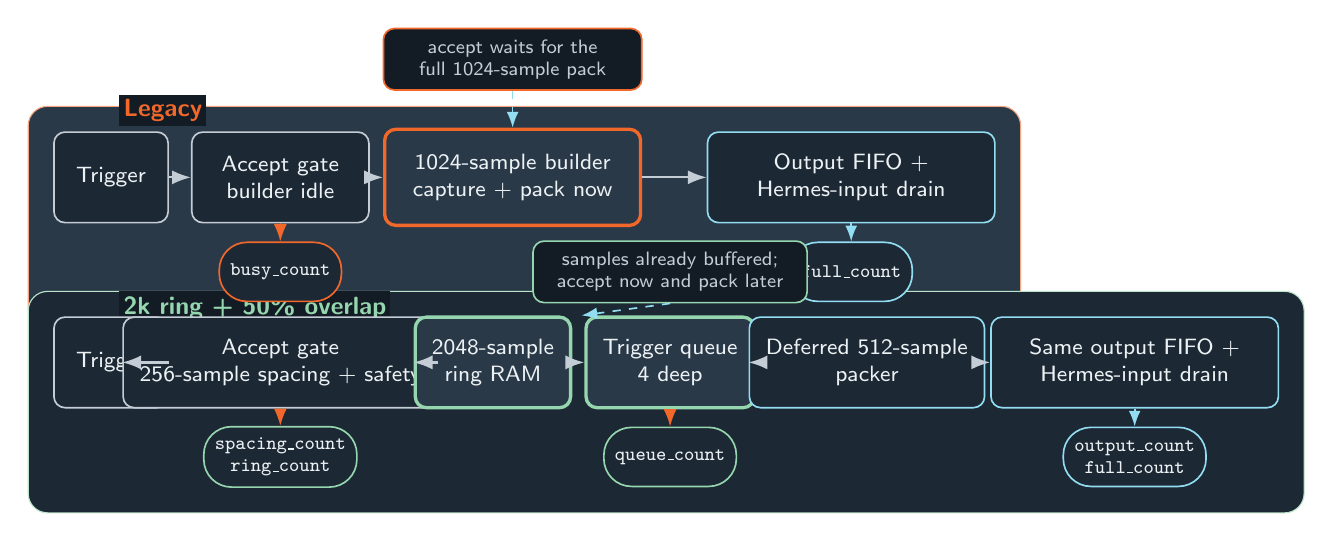
\begin{tikzpicture}[x=1cm,y=1cm]

\node[rowlabel, text=duneorange, anchor=west] at (0.10,4.20) {Legacy};
\node[rowlabel, text=noirmint, anchor=west] at (0.10,1.70) {2k ring + 50\% overlap};

% Legacy row
\node[stage, minimum width=1.45cm] (larrival) at (0.0,3.35) {Trigger};
\node[stage, minimum width=2.25cm] (lgate) at (2.15,3.35) {Accept gate\\builder idle};
\node[hot, minimum width=3.25cm, minimum height=1.22cm] (lbuild) at (5.10,3.35) {1024-sample builder\\capture + pack now};
\node[shared, minimum width=3.65cm] (lout) at (9.40,3.35) {Output FIFO +\\Hermes-input drain};

\draw[flow] (larrival) -- (lgate);
\draw[flow] (lgate) -- (lbuild);
\draw[flow] (lbuild) -- (lout);

\node[reject, draw=duneorange] (lbusy) at (2.15,2.15) {\texttt{busy\_count}};
\node[reject, draw=noircyan] (lfull) at (9.40,2.15) {\texttt{full\_count}};
\draw[accent] (lgate.south) -- (lbusy.north);
\draw[subtle] (lout.south) -- (lfull.north);

\node[callout, draw=duneorange, text width=3.0cm] (lcall) at (5.10,4.85) {accept waits for the full 1024-sample pack};
\draw[subtle] (lcall.south) -- (lbuild.north);

% Ring row
\node[stage, minimum width=1.45cm] (rarrival) at (0.0,1.00) {Trigger};
\node[stage, minimum width=2.25cm] (rgate) at (2.15,1.00) {Accept gate\\256-sample spacing + safety};
\node[future, minimum width=1.95cm] (rring) at (4.85,1.00) {2048-sample\\ring RAM};
\node[future, minimum width=1.75cm] (rqueue) at (7.10,1.00) {Trigger queue\\4 deep};
\node[shared, minimum width=2.20cm] (rpack) at (9.60,1.00) {Deferred 512-sample\\packer};
\node[shared, minimum width=3.65cm] (rout) at (13.00,1.00) {Same output FIFO +\\Hermes-input drain};

\draw[flow] (rarrival) -- (rgate);
\draw[flow] (rgate) -- (rring);
\draw[flow] (rring) -- (rqueue);
\draw[flow] (rqueue) -- (rpack);
\draw[flow] (rpack) -- (rout);

\node[reject, draw=noirmint] (rspace) at (2.15,-0.20) {\texttt{spacing\_count}\\\texttt{ring\_count}};
\node[reject, draw=noirmint] (rqueuecount) at (7.10,-0.20) {\texttt{queue\_count}};
\node[reject, draw=noircyan] (rfull) at (13.00,-0.20) {\texttt{output\_count}\\\texttt{full\_count}};
\draw[accent] (rgate.south) -- (rspace.north);
\draw[accent] (rqueue.south) -- (rqueuecount.north);
\draw[subtle] (rout.south) -- (rfull.north);

\node[callout, draw=noirmint, text width=3.2cm] (rcall) at (7.10,2.15) {samples already buffered; accept now and pack later};
\draw[subtle] (rcall.south) -- ($(rring.north)!0.5!(rqueue.north)$);

\begin{pgfonlayer}{background}
  \node[
    draw=duneorange!60,
    rounded corners=7pt,
    fill=noirpanelalt,
    fit=(larrival)(lout)(lbusy)(lfull),
    inner sep=9pt
  ] {};
  \node[
    draw=noirmint!65,
    rounded corners=7pt,
    fill=noirpanel,
    fit=(rarrival)(rout)(rspace)(rqueuecount)(rfull),
    inner sep=9pt
  ] {};
\end{pgfonlayer}

\end{tikzpicture}
\end{document}
